\documentclass[10pt,a4paper]{article}
\usepackage{tikz} % for drawing figures
\usepackage{amsmath} % for equations
\usepackage{url} % for URLs
\usepackage{graphicx}
\usepackage{multicol}
\usepackage{varwidth}
\usepackage{blindtext}


\usepackage{linguex} % ** special include in directory: for doing handy example labeling and bracketing
\renewcommand{\firstrefdash}{} % used for linguex package not to put hyphens in example refs (1a instead of 1-a)
\usepackage{cogsci}
\usepackage{pslatex}
\usepackage{apacite}

\newcommand{\sem}[1]{\mbox{$[\![$#1$]\!]$}}
\newcommand{\lam}{$\lambda$}
\newcommand{\gcs}[1]{\textcolor{blue}{[gcs: #1]}} 



\title{On the added informativity of ambiguous language}
\author{\large \textbf{our names}\\
our emails\\
our affiliations}


\begin{document}
\maketitle

\begin{abstract}
XXX


\textbf{Keywords:} 
ambiguity, pragmatics, informativity, Rational Speech Act models

\end{abstract}

\section{Introduction}

Linguists often treat ambiguity as a bug in the communication system, something to be avoided or explained away \cite{grice1975,chomsky2002minimalism}. However, recent research has begun to take notice of the efficiency ambiguity affords us: by relying on context to fill in missing information, we can reuse lightweight bits of language rather than fully specifying the intended message \cite{levinson2000,piantadosietal2012,wasow2015}. In other words, ambiguity serves as a feature---not a bug---of an efficient communication system. This reasoning accords with years of psycholinguistic research documenting that speakers readily produce ambiguous utterances (see \citeNP{ferreira2008}, for an overview). 

Moreover, \citeA{wasow2015} reviews a large body of evidence and concludes that ambiguity is rarely avoided, even in situations where it would be communicatively appropriate. While this observation contradicts the Gricean maxim to avoid ambiguity (\citeNP{grice1975}), \citeauthor{wasow2015} points out that \citeauthor{grice1975} was primarily concerned with cases of deliberate ambiguity. In such cases, the recognition of the ambiguity is the communicative purpose. \citeauthor{wasow2015} on the other hand reviews cases where ambiguity production serves no obvious communicative purpose and triggers no implicatures. 

The current work identifies an additional benefit afforded by using ambiguous language: the \emph{extra} information we gain from observing how our listeners resolve ambiguity. We advance the hypothesis that language users learn about each other's private knowledge by observing how they resolve ambiguity. If language does not do the job of specifying the information necessary for full interpretation, then listeners are left to draw on their beliefs and preferences to fill in the gaps; by observing how listeners fill those gaps in, speakers learn about the beliefs and preferences the listeners are using. 

By way of illustration, take, for example, the scenario in Fig.~\ref{FG-ref-game}. Suppose a speaker produces the single-word utterance ``blue'' in an attempt to signal one of the objects to a listener. The utterance is ambiguous; it can pick out either the blue square or the blue circle. Suppose further that, upon hearing ``blue,'' the listener selects the blue circle. In observing this choice, the speaker stands to learn something about the private thoughts of the listener: what made her select the blue circle instead of the blue square? Perhaps the circle is more salient to the listener, or the listener has a preference for circles, or the listener believes the speaker has a preference for circles. By observing how the listener resolves the ambiguity in reference, the speaker can learn this information. 

\begin{figure}
	\centering
	
\includegraphics[width=2in]{images/rsascene.eps}
	\caption{A simple reference game scenario from \citeA{frankgoodman2012}. In the game, speakers choose a single-word utterance to signal one of the objects to a listener. In this scenario, the speaker chooses between the utterances ``blue,'' ``green,'' ``square,'' and ``circle.''}\label{FG-ref-game}
\end{figure}

However, accessing this added information requires the speaker to reason pragmatically about the pragmatic reasoning of the listener---a higher-order pragmatic reasoning, as it were. In order select a referent, the listener must interpret the utterance. We follow \citeA{frankgoodman2012} in treating this interpretation process as active pragmatic reasoning: the listener interprets the utterance by reasoning about the process that generated it, namely the speaker, who selects as utterance by reasoning about how a listener would interpret it. \citeauthor{frankgoodman2012} model this recursive social reasoning between speakers and listeners; their model serves as the launch point for the Rational Speech Act (RSA) modeling framework.

The current paper builds on the foundational, vanilla RSA model of reference games by introducing uncertainty about the prior beliefs of the listener and modeling a speaker who reasons about these beliefs on the basis of the observed referent choice. We begin by walking through our modeling assumptions, then presenting our model in full detail. We then test the behavioral predictions of our model against human data in a series of web-based experiments. We conclude with a discussion of the significance of our findings for understanding ambiguity in natural language.


\section{Model}

We begin with the vanilla RSA model of \citeA{frankgoodman2012}. The recursive social reasoning inherent to the RSA modeling framework gets cashed out as various layers of inference. At the base, there is a hypothetical, naive literal listener $L_0$ who hears an utterance $u$ and infers the state of the world $s$ that utterance is meant to describe. $L_0$ performs this inference by conditioning on the literal semantics of $u$, \sem{$u$}. $L_0$ thus returns a uniform distribution over those states $s$ that can be truthfully described by $u$:
$$P_{L_{0}}(s|u) \propto \sem{$u$}(s).$$
One layer up, the speaker $S_1$ observes some state $s$ and chooses an utterance $u$ to communicate that state to $L_0$. $S_1$ chooses utterances on the basis of their utility for signaling $s$ to $L_0$, $U_{S_1}(u;s)$. The speaker's utility maximizes the probability that $L_0$ would arrive at the correct $s$ on the basis of $u$, $P_{L_{0}}(s|u)$, while minimizing the cost of $u$ itself, $C(u)$:
$$U_{S_{1}}(u;s) = \textrm{log}(P_{L_{0}}(s|u)) - C(u).$$
$S_1$ chooses utterances in proportion to their utility:
$$P_{S_{1}} (u|s) \propto   \textrm{exp}(\alpha \cdot U_{S_{1}} (u;s)).$$
At the top layer of inference, the \emph{pragmatic} listener $L_1$ infers $s$ on the basis of some observed $u$. The result is a distribution over likely states $s$; however, unlike $L_0$, $L_1$ updates beliefs about the world by reasoning about the process that \emph{generated} $u$, namely $S_1$. In other words, $L_1$ reasons about the $s$ that would have been most likely to lead $S_1$ to choose the  $u$ that was observed:
$$P_{L_{1}}(s|u) \propto P_{S_{1}}(u|s) \cdot P(s).$$

\citeA{frankgoodman2012} test the predictions of their model against behavioral data from reference games as in Figure \ref{FG-ref-game}. To model production behavior---which utterance should be chosen to communicate a given object---the authors generate predictions from $S_1$. To model interpretation behavior---which object is the speaker trying to communicate on the basis of their utterance---the authors generate predictions from $L_1$. Finding extremely high correlations between model predictions and behavioral data in both cases, \citeauthor{frankgoodman2012} have strong support for their model of pragmatic reasoning in reference games (see also \citeNP{qingfranke2015}, for a fuller exploration of the modeling choices).

Our model builds on the vanilla version of RSA above by allowing for uncertainty around the listener's state prior, $P(s)$. We have in mind a scenario where a listener might have a preference for a certain object features (e.g., blue things, squares, circles, etc.), and these preference will influence their object choice. With this in mind, speaker produces an utterance, observes the listener's referent choice, and, on the basis of that choice, infers the preferences the listener might have had when making it. We use the same $L_0$ and $S_1$ from the vanilla model. However, we now parameterize $L_1$'s state prior so that it operates with respect to a given feature preference $P(s|f)$:
$$P_{L_{1}}(s|u,f) \propto P_{S_{1}}(u|s) \cdot P(s|f).$$
We then model a pragmatic speaker $S_2$ who updates beliefs about $L_1$'s preferences, $P(f)$. To do so, $S_2$ produces $u$ and observes $L_1$'s choice of $s$, then reasons about the feature preference $f$ that $L_1$ used to make that choice:
$$P_{S_{2}}(f|u,s) \propto P_{L_{1}}(s|u,f) \cdot P(f).$$
We can also model the reasoning process by which a speaker selects the best utterance to learn about the preferences of the listener. Starting with no knowledge of the listener's preferences, $S_2$ will have a uniform (i.e., flat) feature preference prior $P(f)$; to the extent that the speaker's posterior beliefs about the preferences, $P_{S_{2}}(f|u,s)$, deviate from the uniform prior, the speaker will have learned something about listener preferences. Thus, we can model the reasoning behind strategic utterance selection as an attempt to maximize the KL divergence between speaker's prior and their posterior, summing over the possible feature preferences $f$ and state observations $s$:
$$P_{b}(u) \propto \sum_{s:\  [\![u]\!](s)}\textrm{KL}(P(f),P_{S_{2}}(f|u,s))-C(u).$$

We now have two sets of predictions from our model to check: first, pragmatic speaker predictions for inferring listener feature preferences on the basis of their object choice; and second, strategic utterance selection predictions for choosing the best utterance to learn about listener preferences. Below, we present two experiments that test these predictions against human behavior.


\section{Expt.~1: Inferring preferences}

Our first task is to check the predictions of our $S_2$ layer: having observed that a listener selects some referent $s$ in response to an utterance $u$, what are the most likely preferences the listener had when making their choice? 

\subsection{Participants}

We recruited XX participants with US IP addresses through Amazon.com's Mechanical Turk crowdsourcing service. Participants received \$XXX for their participation. On the basis of a post-test demographics questionnaire, we identified XXX participants as native speakers of English; their data were included in the analyses reported below.

\subsection{Design and methods}

We presented participants with a series of reference game scenarios modeled after Figure \ref{FG-ref-game} from \citeA{frankgoodman2012}. Each scenario featured two people and three objects. One of the people served as the speaker, and the other served as the listener. The speaker asks the listener to choose one of the objects, but in doing so she is allowed to mention only one of the features of the target object. Participants were told that the listener might have a preference for certain object features, and participants were tasked with inferring those preferences after observing the speaker's utterance and listener's object choice.

We followed \citeA{frankgoodman2012} in our stimuli creation. Objects were allowed to vary along three dimensions: color (blue, red, green), shape (cloud, circle, or square), and pattern (solid, striped, polka-dotted). Speaker and listener names were chosen at random on each trial. Participants saw the speaker's utterance in bold (e.g., ``green'' in Figure \ref{exp1-trial}) and the listener's choice appeared with a dotted orange outline (e.g., the leftmost object in Figure \ref{exp1-trial}). Based on the observed choice, participants were instructed to adjust a series of six sliders to indicate how likely it is that the listener had a preference for a given feature. The six features were chosen from the feature dimension that was not mentioned in the speaker's utterance (e.g., pattern and shape in Figure \ref{exp1-trial}). Participants completed a series of XXX trials. Objects and utterances were chosen at random, with the constraint that XXX trials were potentially informative with respect to listener preferences and XXX trials were uninformative with respect to listener preferences (e.g., observing that the listener chose one of three identical objects). 

\begin{figure*}[ht]
	\centering
	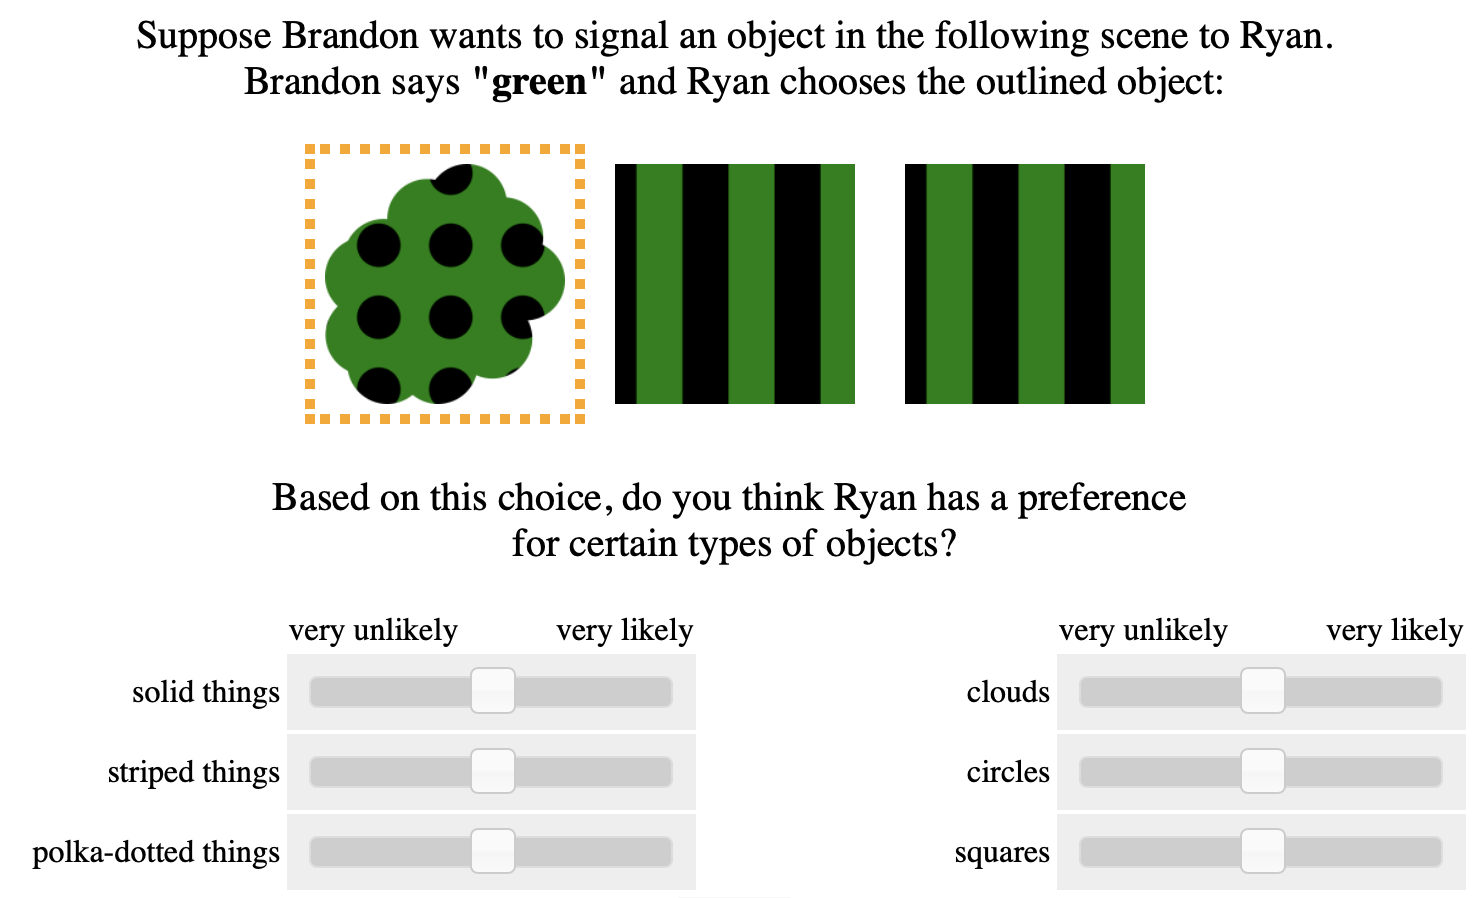
\includegraphics[width=4.5in]{images/exp1-trial.eps}
	\caption{A sample trial from \emph{Experiment 1: Inferring preferences}.}\label{exp1-trial}
\end{figure*}

\subsection{Results and discussion}

XXX something about the data processing

XXX something about model fitting

XXX something about comparing between human and model


\section{Expt.~2: Choosing utterances}

Our next task is the check the predictions of our strategic utterance selection model: given a set of potential referents, which utterance would be most informative with respect to the listener's preferences?

\subsection{Participants}

We recruited XX participants with US IP addresses through Amazon.com's Mechanical Turk crowdsourcing service. Participants received \$XXX for their participation. On the basis of a post-test demographics questionnaire, we identified XXX participants as native speakers of English; their data were included in the analyses reported below.

\subsection{Design and methods}

Participants encountered a reference game scenario similar to Experiment 1 in which a speaker signals an object to a listener who might have a preference for certain types of objects. However, rather than observing the utterance and referent choice, participants were now tasked with helping the speaker choose an utterance that was ``most likely to reveal the listener's color, shape, or pattern preferences.''

We used the same sets of objects from Experiment 1, which could vary along three dimensions. Each trial featured a set of three objects, as in Figure \ref{exp2-trial}. After observing the objects, participants adjusted sliders to indicate which single-feature utterance the speaker should choose. Potential utterances corresponded to the features of the objects present; depending on the number of unique features, participants adjusted between three and nine sliders. Participants completed a series of XXX trials. As with Experiment 1, objects were chosen at random, with the constraint that XXX trials were potentially informative with respect to listener preferences (as in Figure \ref{exp2-trial}) and XXX trials were uninformative with respect to listener preferences (e.g., observing a set of three identical objects). 

\begin{figure*}[ht]
	\centering
	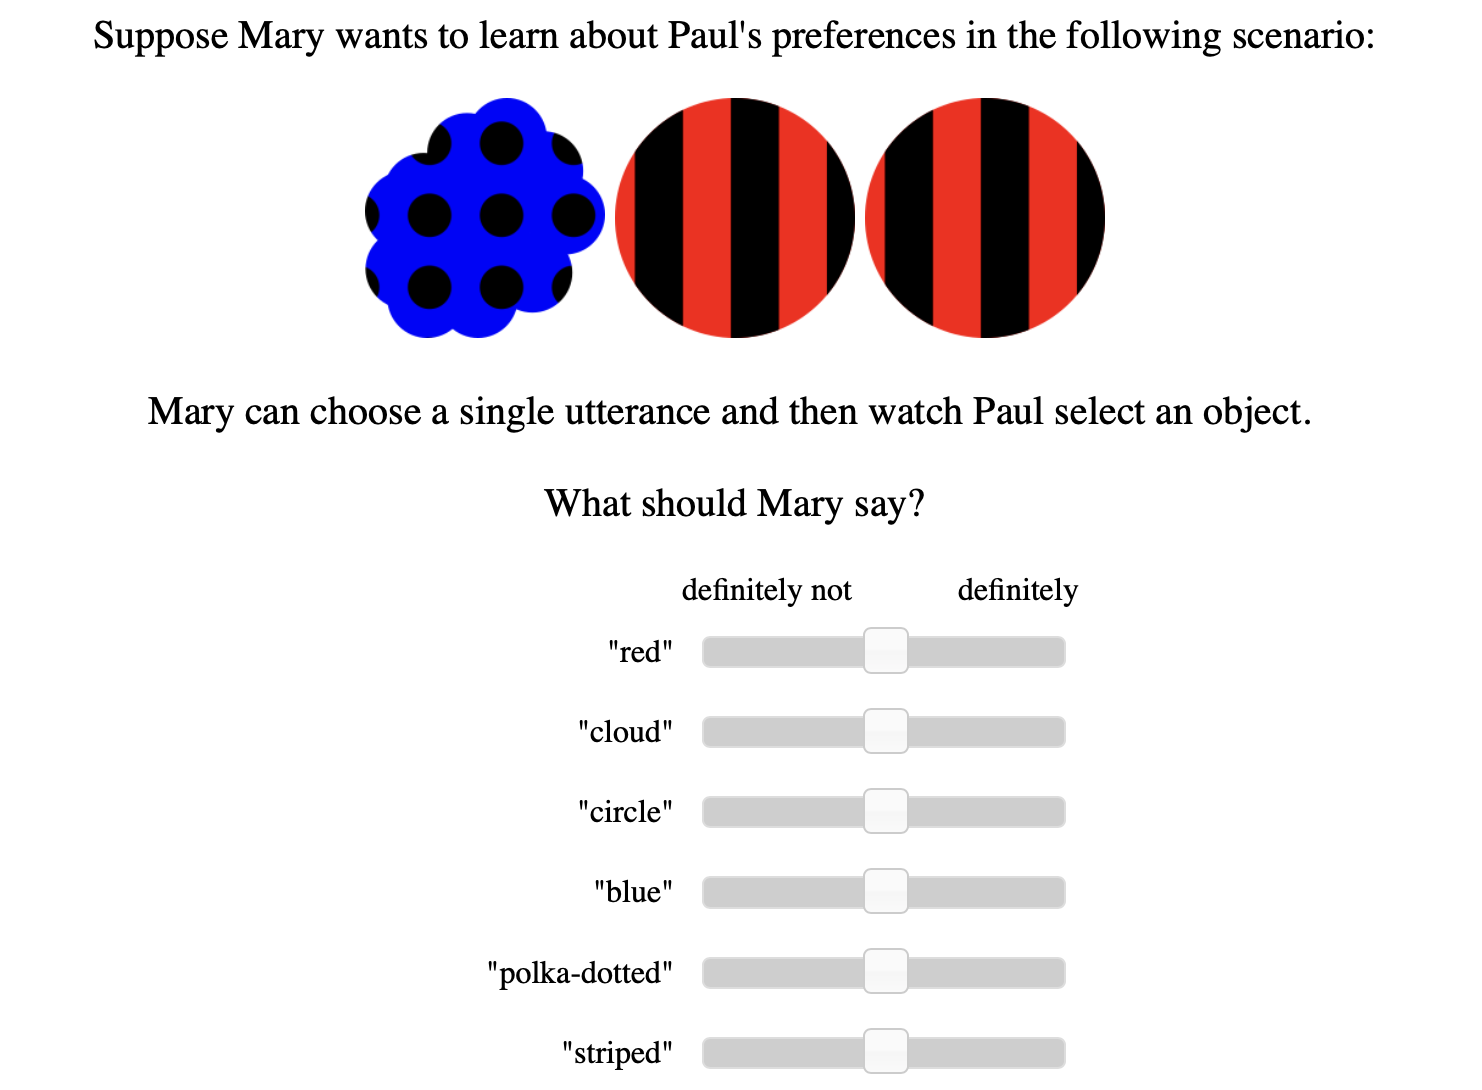
\includegraphics[width=4.5in]{images/exp2-trial.eps}
	\caption{A sample trial from \emph{Experiment 2: Choosing utterances}.}\label{exp2-trial}
\end{figure*}

\subsection{Results and discussion}

XXX something about the data processing

XXX something about model fitting

XXX something about comparing between human and model

\section{Discussion}

We have found strong support for our model of inferring priors on the basis of ambiguous language. The results of Experiment 1 demonstrate that naive speakers are able to reason pragmatically about \emph{why} listeners might take the actions they do, and the success of our computational model in predicting the observed behavior offers an articulated hypothesis about \emph{how} this reasoning proceeds: when speakers are aware of the ambiguity in their utterances, observing how listeners resolve that ambiguity provides clues to the preferences listeners use when doing so. The results of Experiment 2 demonstrate that speakers are able to capitalize on this reasoning to strategically select utterances that are most likely to inform their understanding of the preferences of their listeners. Crucially, the most informative utterances are also the most ambiguous.


in conversation the priors dynamically unfold according to beliefs and preferences about the world and speakers

twin anecdote, politeness (why not ask directly?)

is ambiguity a feature that evolved under pressure from these considerations (i.e., informing preferences), or did ambiguity predate these considerations and speakers merely figured out clever ways of capitalizing on it---a lemonade-out-of-lemons scenario?

\bibliographystyle{apacite}
\setlength{\bibleftmargin}{.125in}
\setlength{\bibindent}{-\bibleftmargin}

\bibliography{prior-inference}

\end{document}

